\documentclass{article}
\usepackage[utf8]{inputenc}

\usepackage[T2A]{fontenc}
\usepackage[utf8]{inputenc}
\usepackage[russian]{babel}

\usepackage{amsmath}
\usepackage[rightcaption]{sidecap}

\usepackage{graphicx} %package to manage images

\usepackage{titlesec}
\setcounter{secnumdepth}{4}
\titleformat{\paragraph}
{\normalfont\normalsize\bfseries}{\theparagraph}{1em}{}
\titlespacing*{\paragraph}
{0pt}{3.25ex plus 1ex minus .2ex}{1.5ex plus .2ex}

\setcounter{tocdepth}{4}
\setcounter{secnumdepth}{4}

\title{Вычислительная техника}
\author{Лисид Лаконский}
\date{October 2022}

\begin{document}

\maketitle
\tableofcontents
\pagebreak

\section{Вычислительная техника - 03.10.2022}

Ревью прошлого зантия: совершенная дизъюнктивная (или) форма, соершенная конъюнктивная (и) нормальная форма, минимазция с помощью трех методов: алгебраического, с помощью карт Карно, с помощью диаграммы Вейча.

\subsection{Табличные методы минимизации}

\subsubsection{Минимизация с помощью карт Карно}

$
\begin{pmatrix}
     & 0 & 1 \\
    0 \\
    1
\end{pmatrix}
$ - шаблон карты Карно для функции, принимающей два аргумента.

$
\begin{pmatrix}
     & 00 & 01 & 11 & 10 \\
    0 \\
    1
\end{pmatrix}
$ - шаблон карты Карно для функции, принимающей три аргумента.

$
\begin{pmatrix}
     & 00 & 01 & 11 & 10 \\
    00 \\
    01 \\
    11 \\
    10
\end{pmatrix}
$ - шаблон карты Карно для функции, принимающей четыре аргумента.

Основные принципы склейки:

\begin{enumerate}
    \item Склейку клеток одной и той же карты Карно можно осуществлять как по единицам (a), так и по нулям (б). Первое необходимо для получения ДНФ, второе — для получения КНФ
    \item Склеивать можно только прямоугольные области с числом единиц (нулей), являющимся целой степенью двойки
    \item Рекомендуется выбирать максимально возможные области склейки
    \item Для карт Карно с числом переменных 3 и 4 применимо следующее правило: крайние клетки каждой горизонтали и каждой вертикали граничат между собой и могут объединяться в прямоугольники (топологически карта Карно представляет собой тор). Следствием этого правила является смежность всех четырёх угловых ячеек карты Карно для 4 переменных
\end{enumerate}

\subsubsection{Минимизация с помощью диаграмм Вейча}

Метод минимизации с помощью диаграмм Вейча основан на методе с применением карт Карно, однако элементы записываются иначе, более удобно для формирования итоговой формулы: лучше смотреть, что изменяется, а что нет.

Все записывается так же с помощью кода Грея, неизменяющиеся элементы подписываются так, чтобы образовывать единицу.

\subsection{Цифровые комбинационные устройства}

\subsubsection{Устройство равнозначности}

$y = (x_{1}x_{2}) + (\overline{x_{1}}\overline{x_{2}}) = \overline{\overline{x_{1}x_{2}} * \overline{\overline{x_1}\overline{x_2}}}$

Возвращает единицу, если оба аргумента равны, иначе ноль.

\subsubsection{Устройство неравнозначности}

$y = x_1\overline{x_2} + \overline{x_1}x_2$

Возвращает единицу, если оба аргумента не равны, иначе ноль.

\subsubsection{Полусумматор}

$S = x_1 \oplus x_2, P = x_{1}x_{2}$

$S$ - сумма, $P$ - перенос

\subsubsection{Комбинационный сумматор}

Комбинационный сумматор, удивительно, получается при помощии комбинации полусумматоров или других сумматоров.

Схемы тут не будет, так как в LaTeX крайне неудобно прикреплять картинки. По крайней мере, мне лень сейчас разбираться, как тут в Overleaf это делать.

Складываются аргументы, а потом результат работы сумматора складывается с переносом.

\pagebreak
\section{Вычислительная техника - 17.10.2022}

\subsection{Шифраторы}

\begin{flushleft}

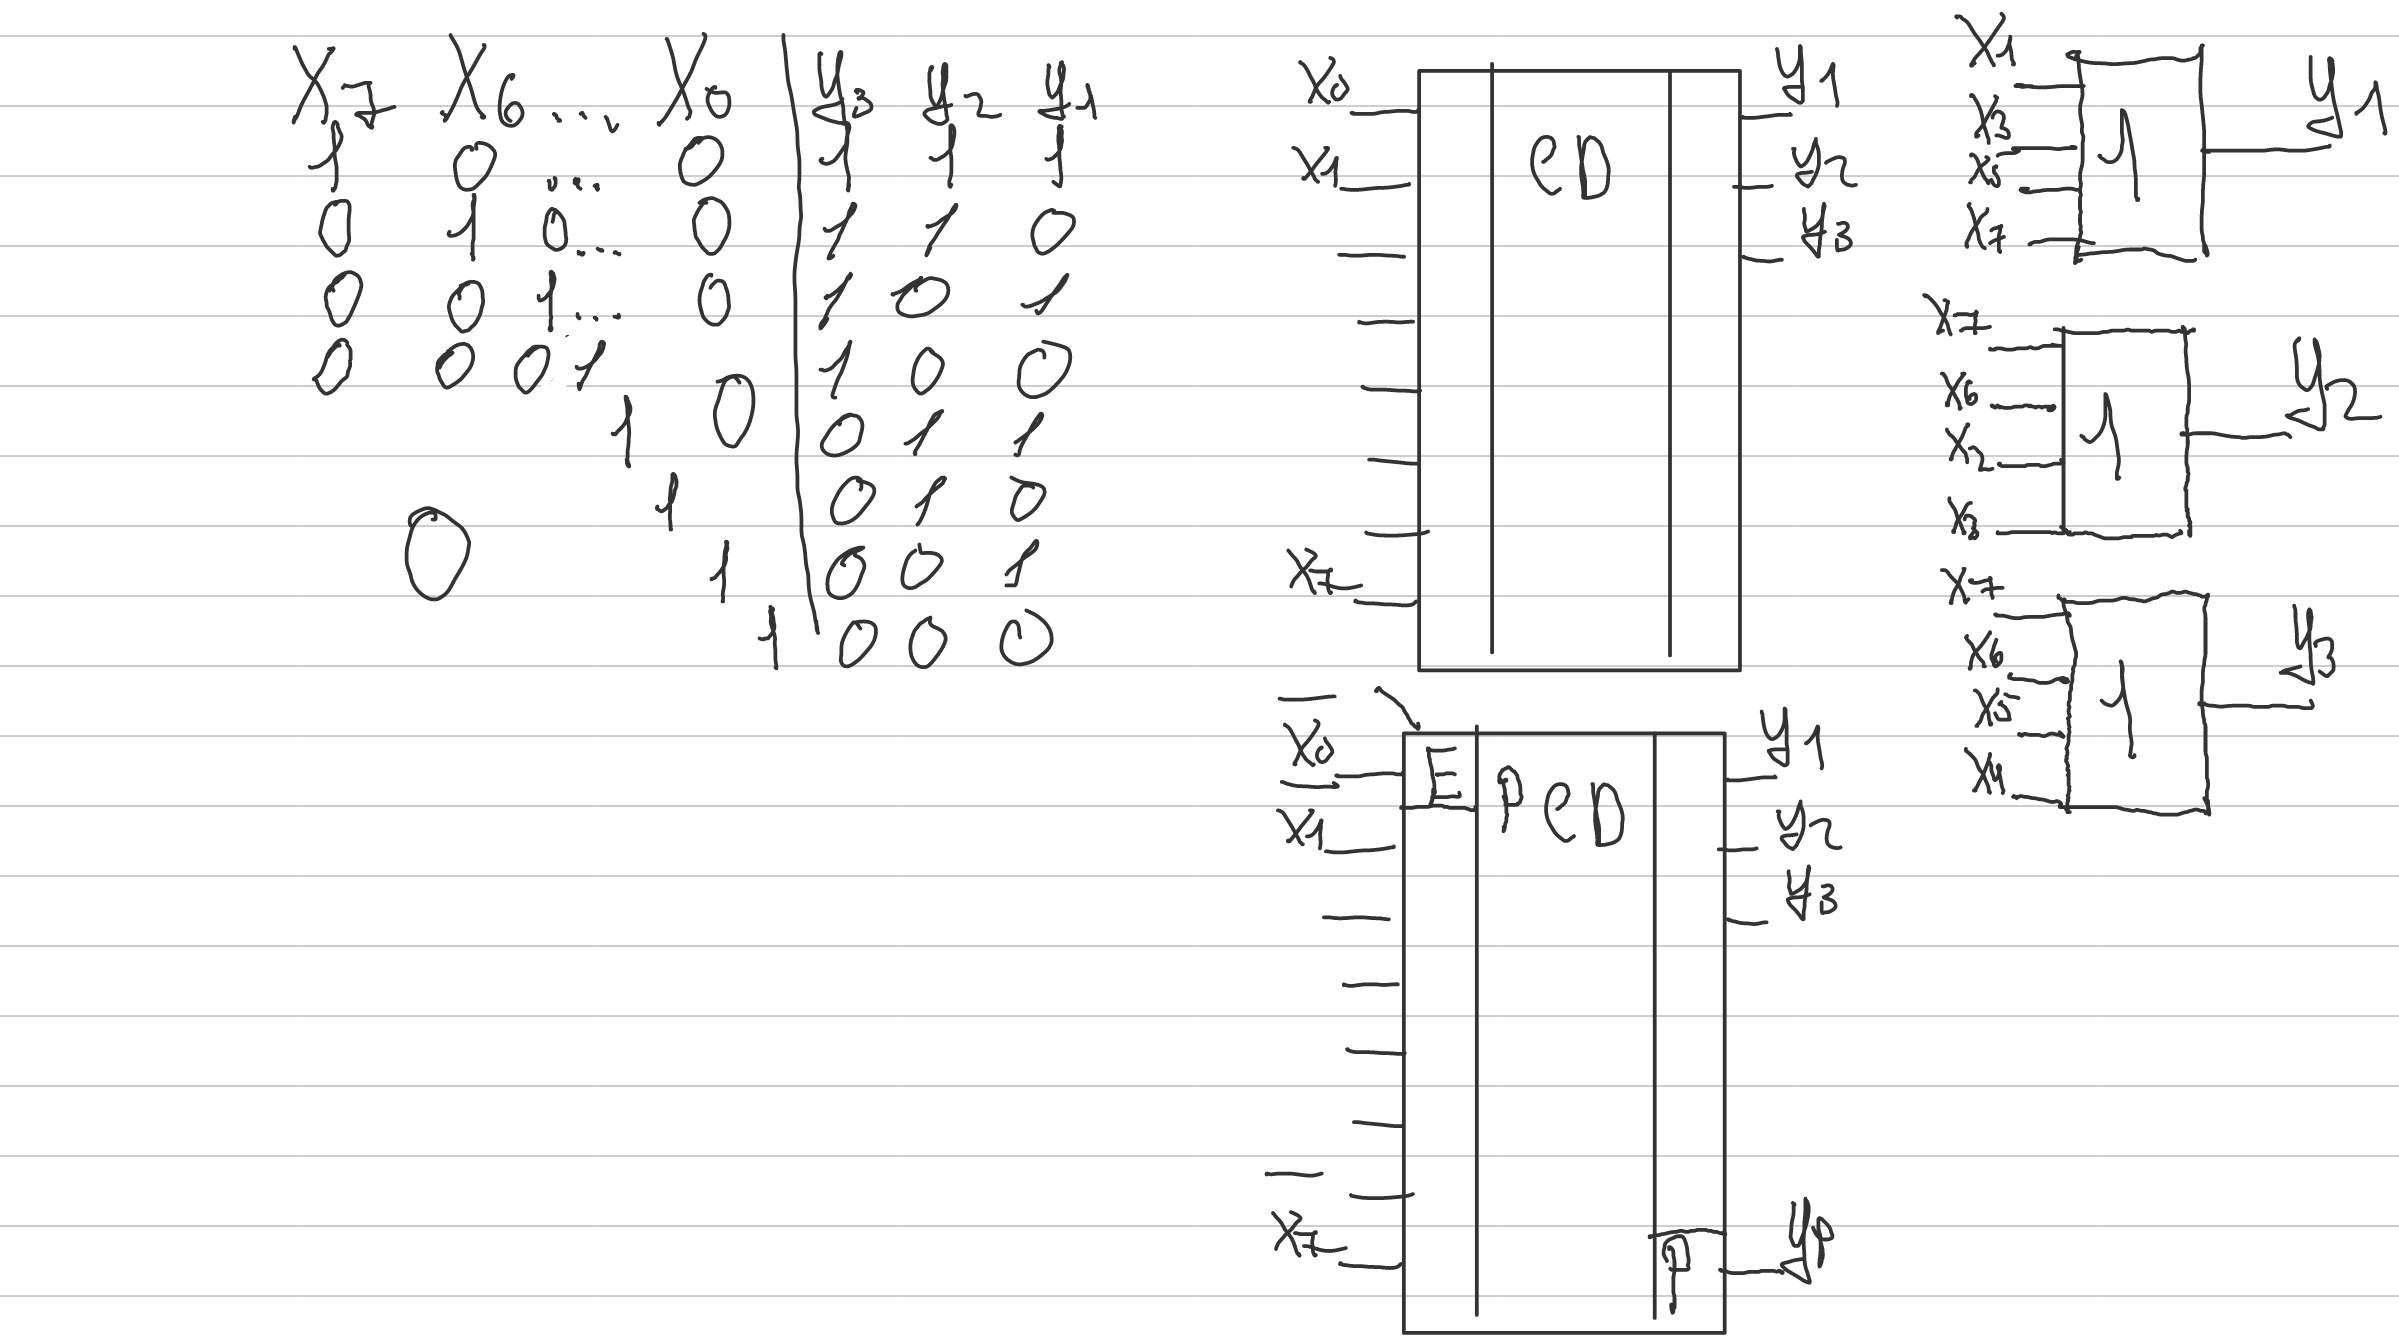
\includegraphics[width=\textwidth]{coder.png}

\subsubsection{Устранение неоднозначности}

Устранять неоднозначность можно с помощью приоритетного шифратора - дополнительный выход $p$ - выход признака невозбуждения: 0 - возбужден хотя бы один из входов, 1 - в противном случае, дополнительный вход $E$.

\subsection{Дешифраторы}

\subsubsection{Линейные дешифраторы}

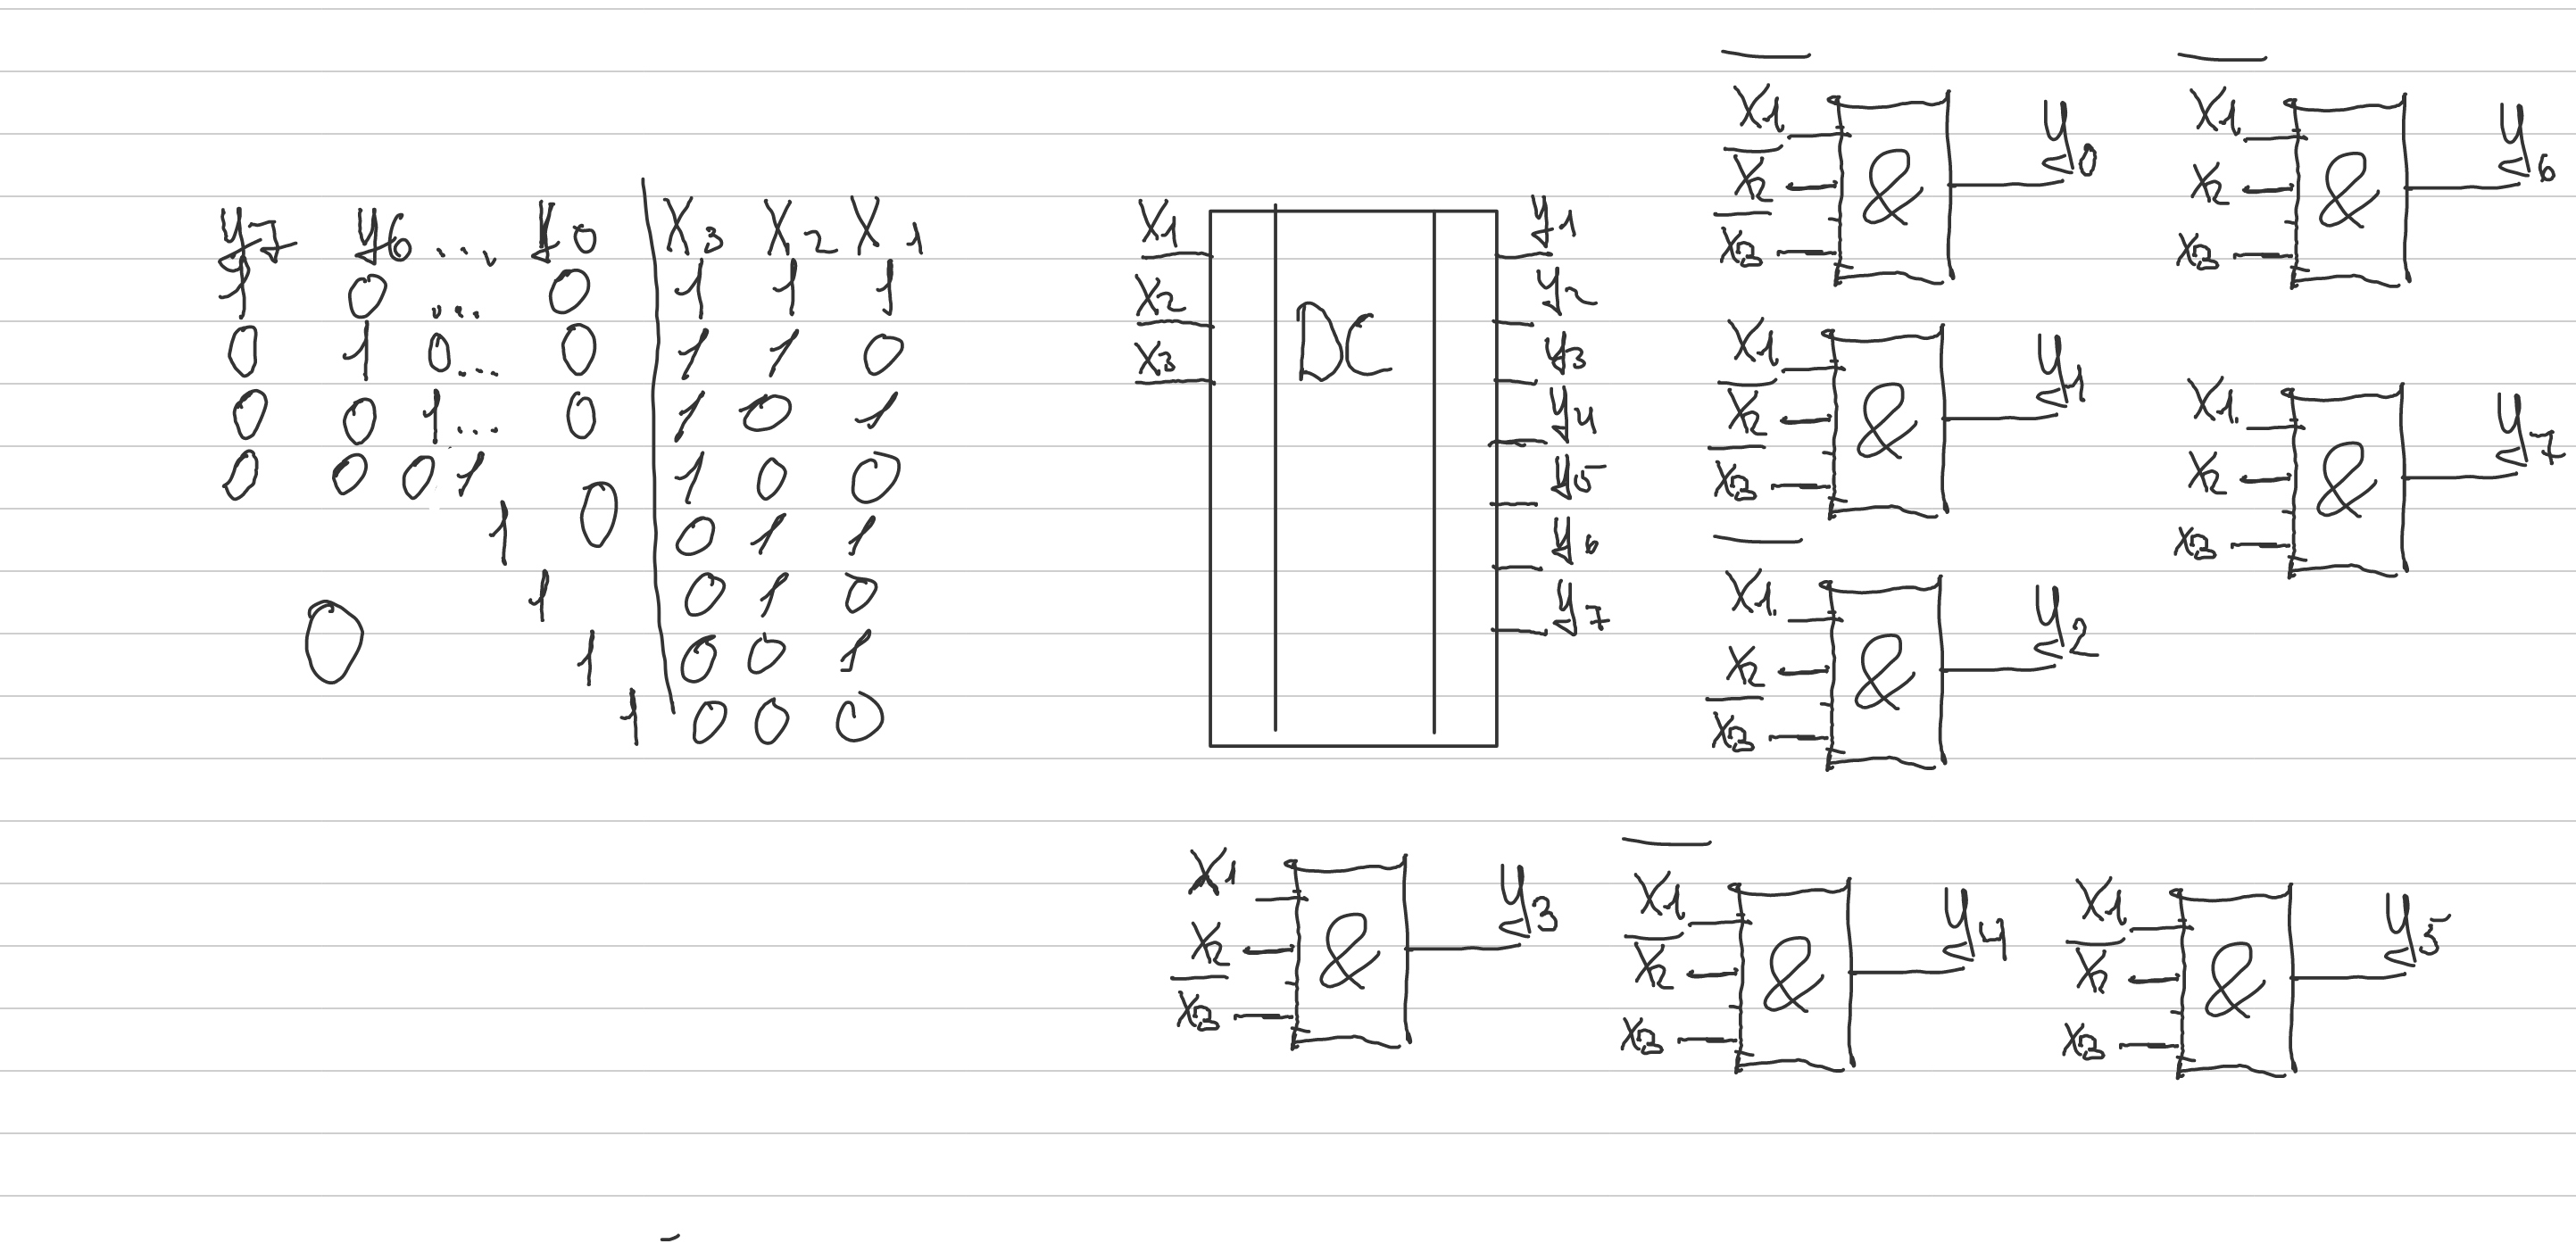
\includegraphics[width=\textwidth]{decoder.png}

\hfill

Ниже приведено обозначение микросхемы К155ИД4

\hfill

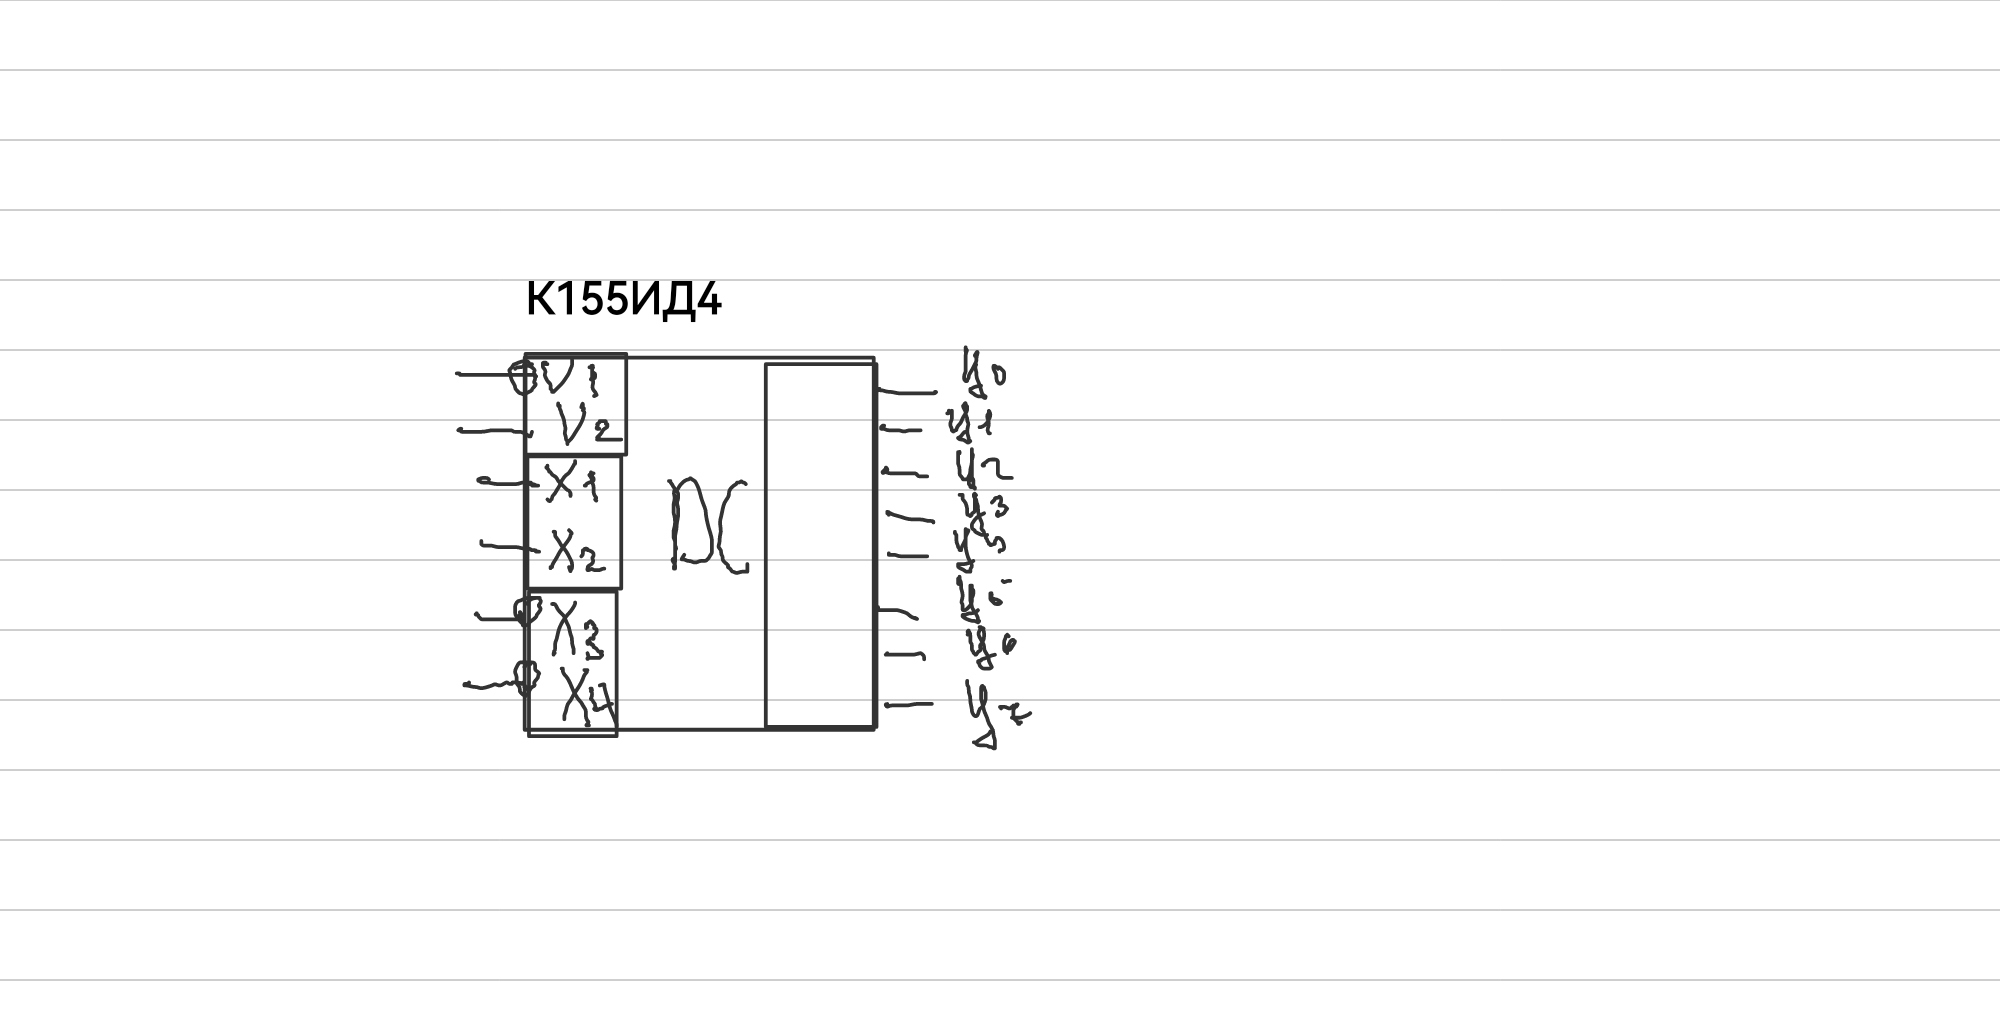
\includegraphics[width=\textwidth]{k155id4.png}

Существуют также пирамидальные, каскадные дешифраторы.

\subsubsection{Каскадный дешифратор}

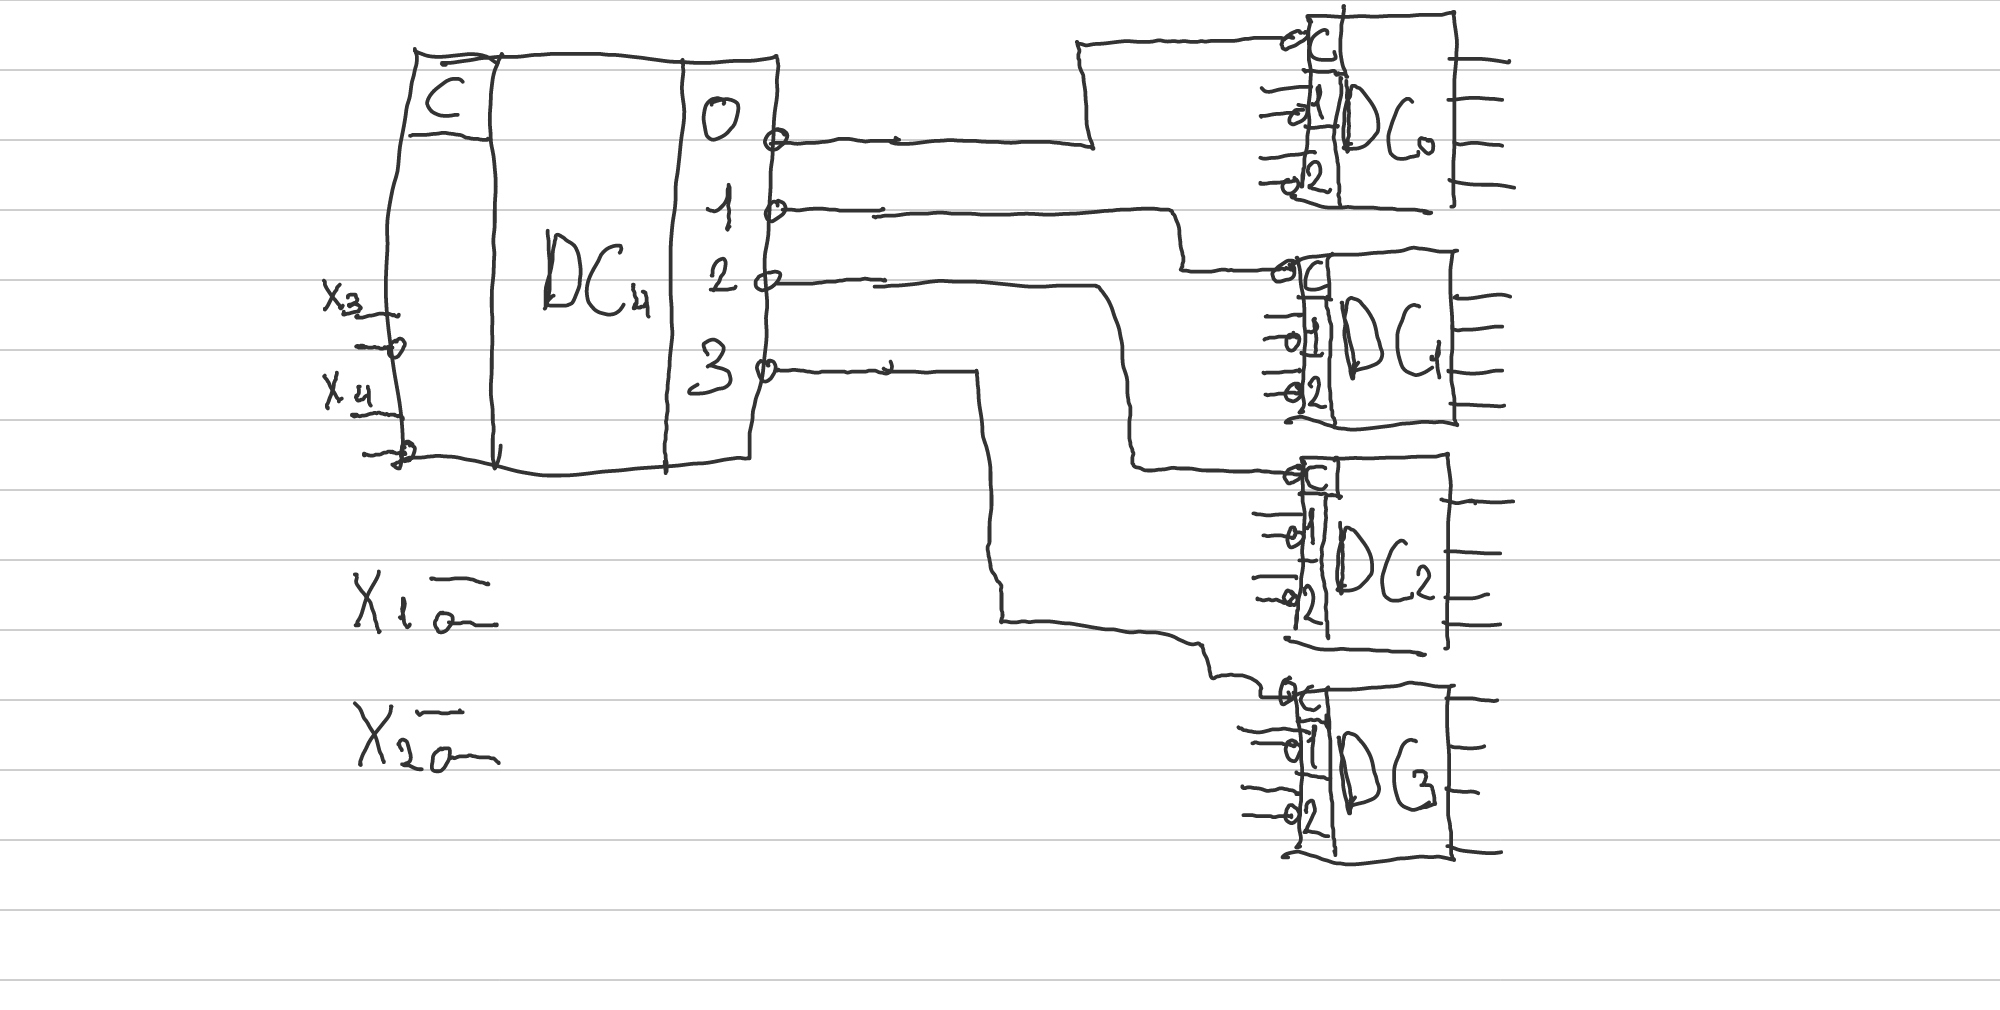
\includegraphics[width=\textwidth]{cascade.png}

\subsection{Мультплексор}

Мультиплексор обеспечивает коммутацию на вход одного из входных сигналов.

Формула:

$y = \overline{x_3}\overline{x_2}\overline{x_1}D_0 + \overline{x_3}\overline{x_2}x_1D_1 + \overline{x_3}x_2\overline{x_1}D_2 + ... + x_3x_2x_1D_7$

\hfill

В формулу может быть добавлен управляющий сигнал:

$y = \overline{x_3}\overline{x_2}\overline{x_1}D_0\overline{v} + \overline{x_3}\overline{x_2}x_1D_1\overline{v} + \overline{x_3}x_2\overline{x_1}D_2\overline{v} + ... + x_3x_2x_1D_7\overline{v}$

\subsubsection{Схема}

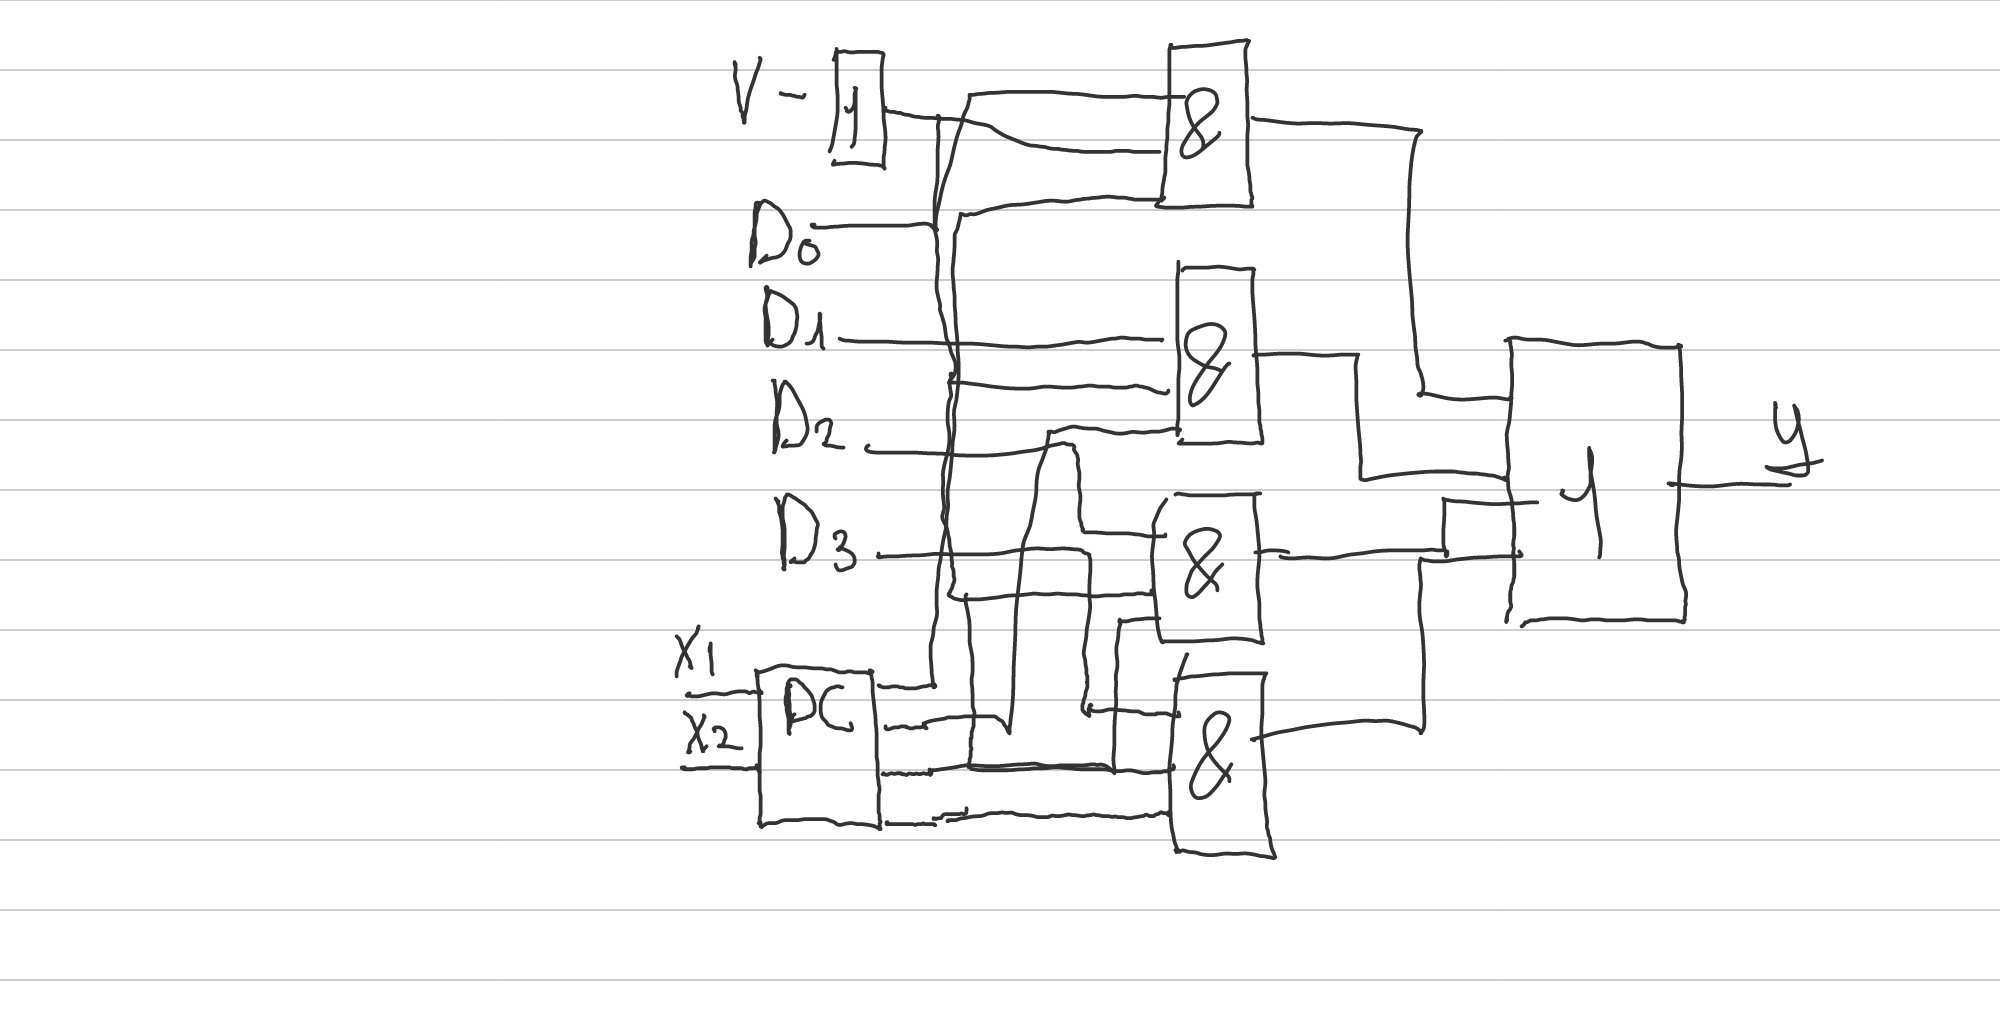
\includegraphics[width=\textwidth]{multiplexer.png}

\subsubsection{Схема в multisim}

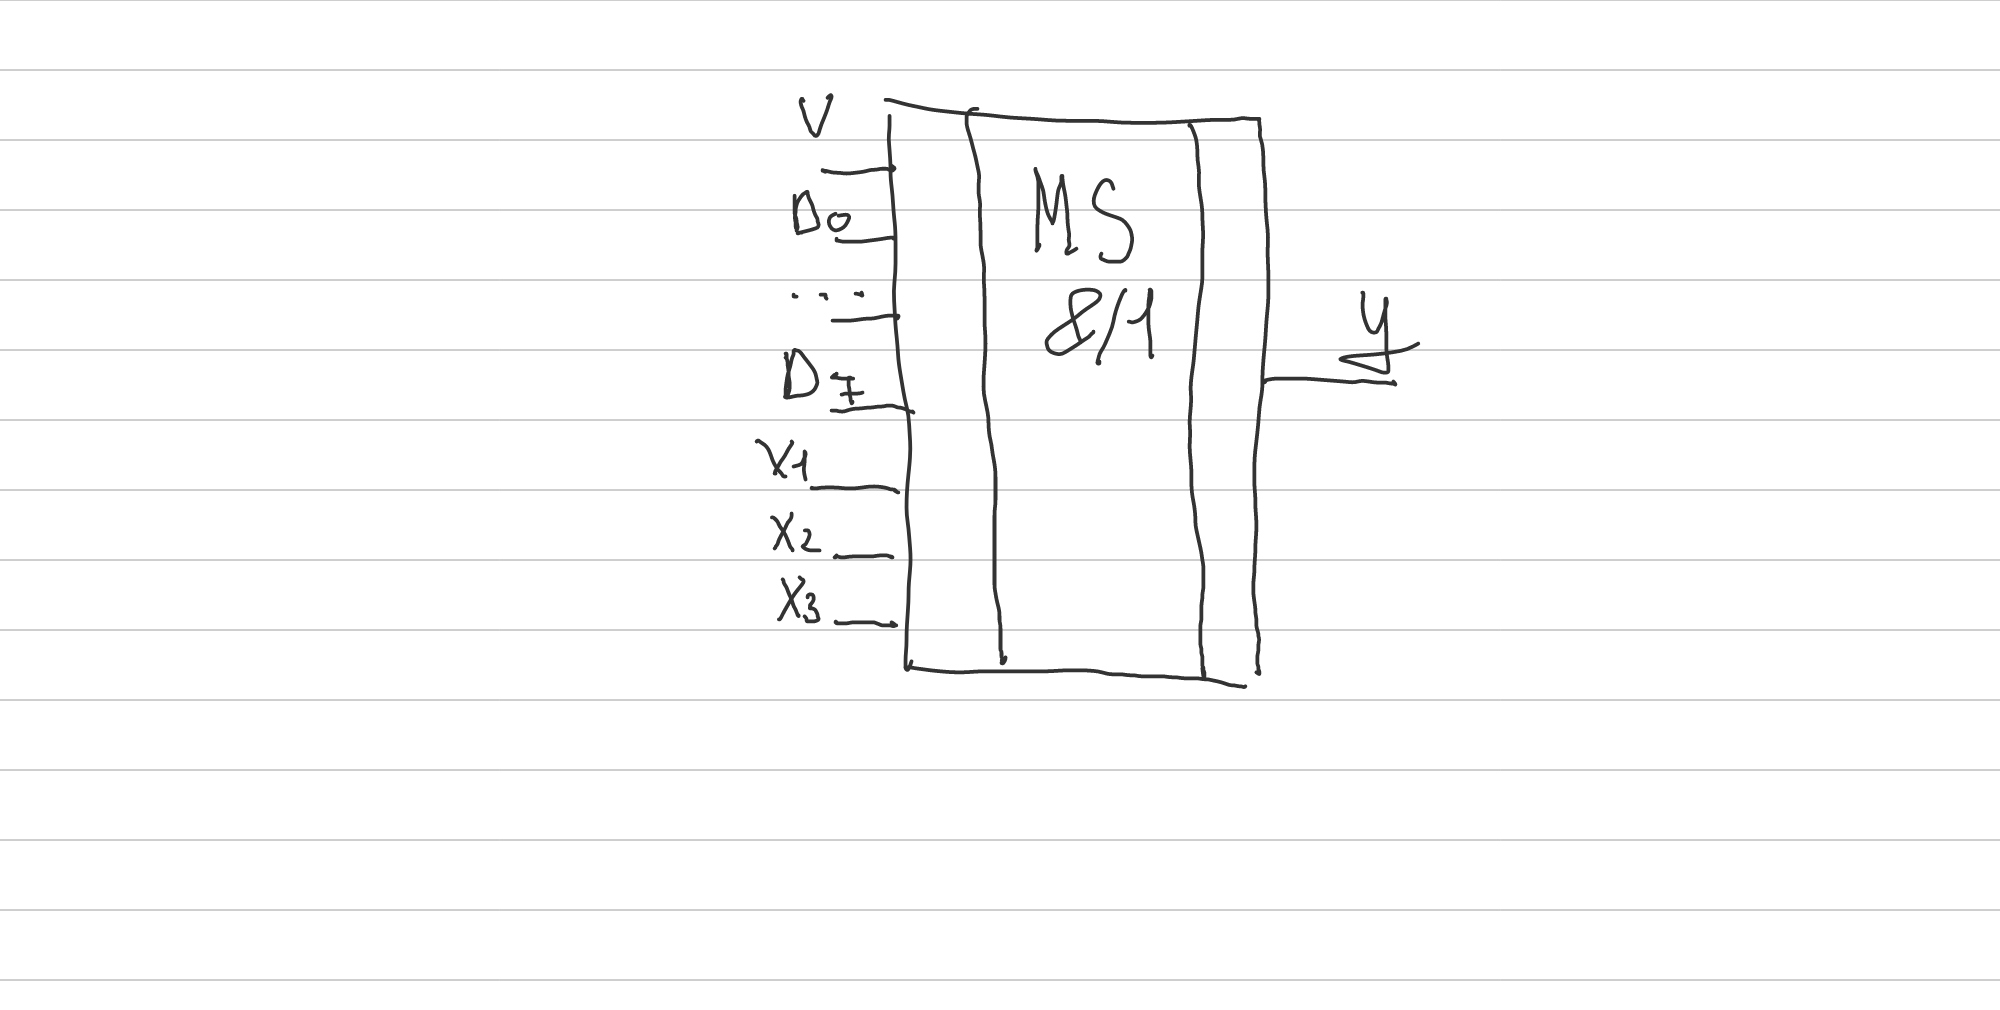
\includegraphics[width=\textwidth]{multiplexer-multisim.png}

\subsection{Демультиплексор}

Демультиплексор — это логическое устройство, предназначенное для переключения сигнала с одного информационного входа на один из информационных выходов.

\hfill

Формула:

$y_0 = \overline{x_2} \overline{x_1} D, y_1 = \overline{x_1}D, y_2 = x_2\overline{x_1}D, y_3 = x_2 x_1 D$

\subsubsection{Схема}

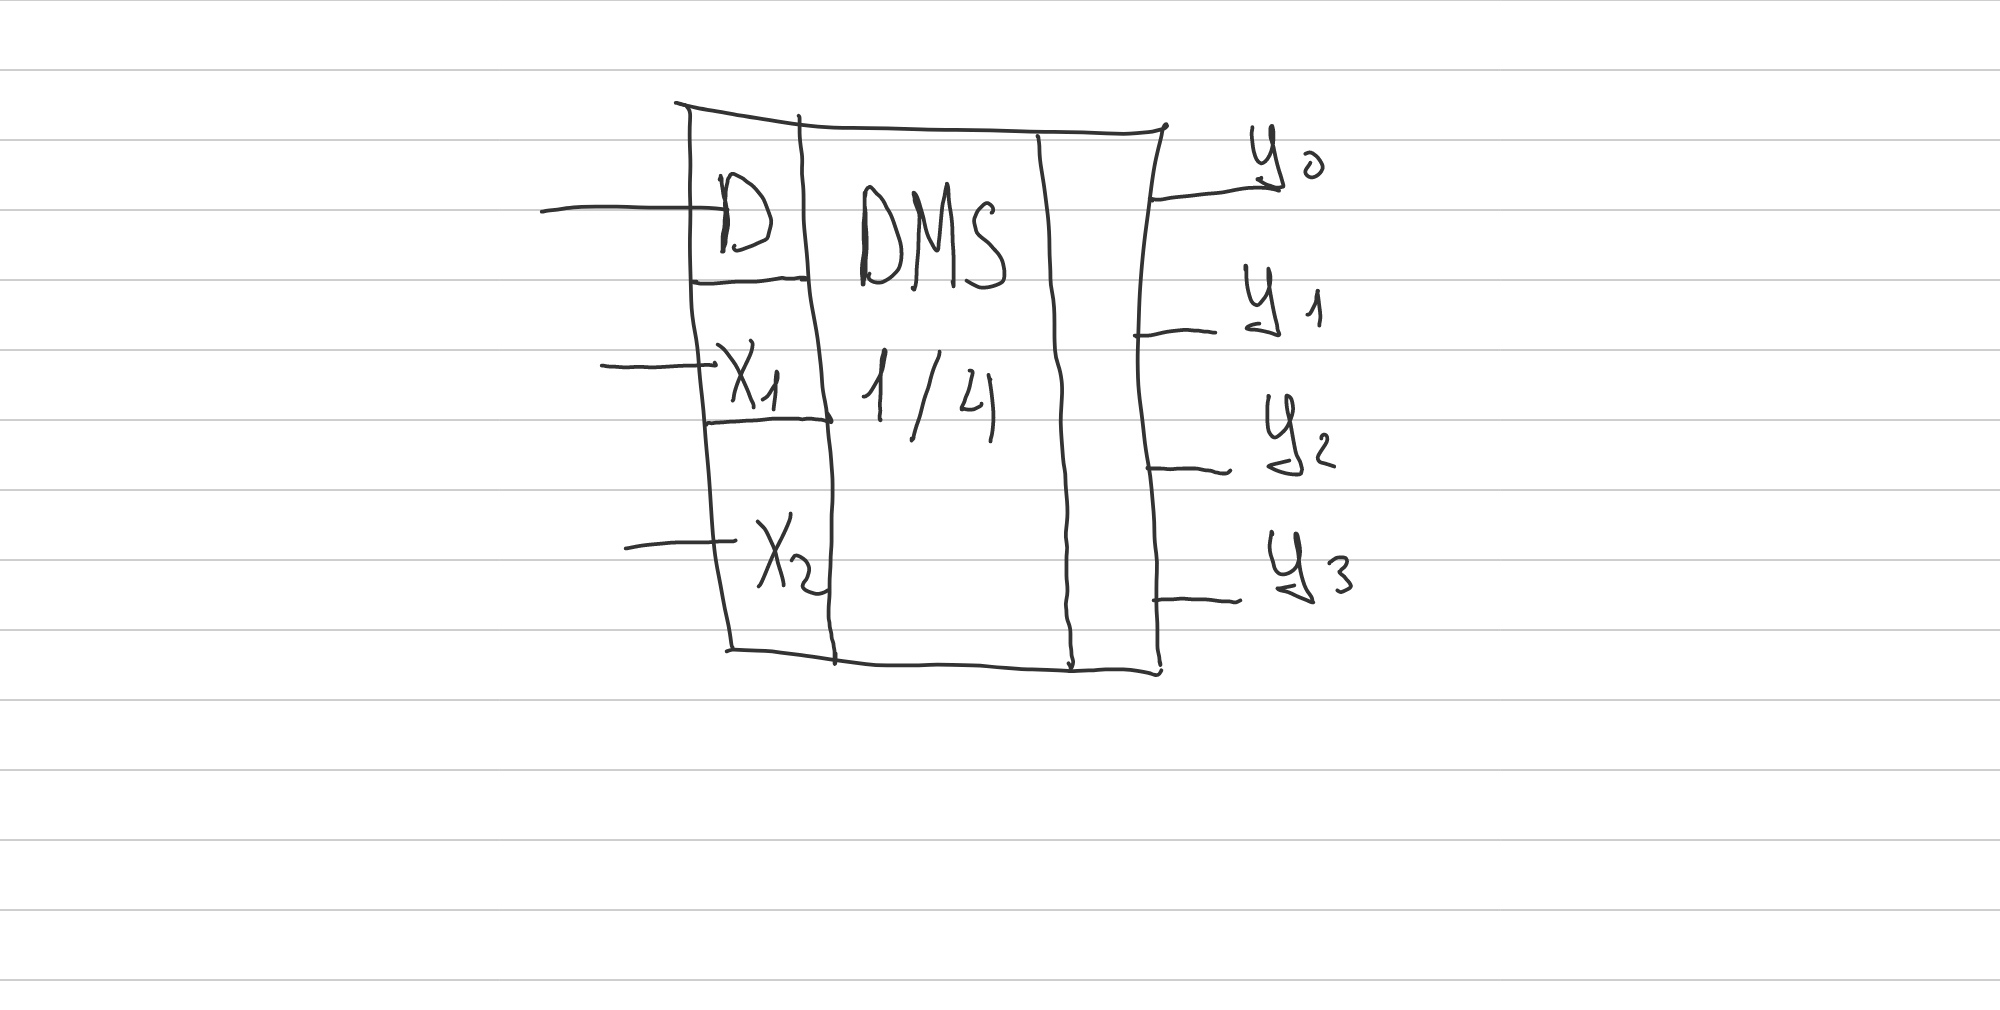
\includegraphics[width=\textwidth]{demultiplexer.png}

\pagebreak
\section{Вычислительная техника - 17.10.2022}

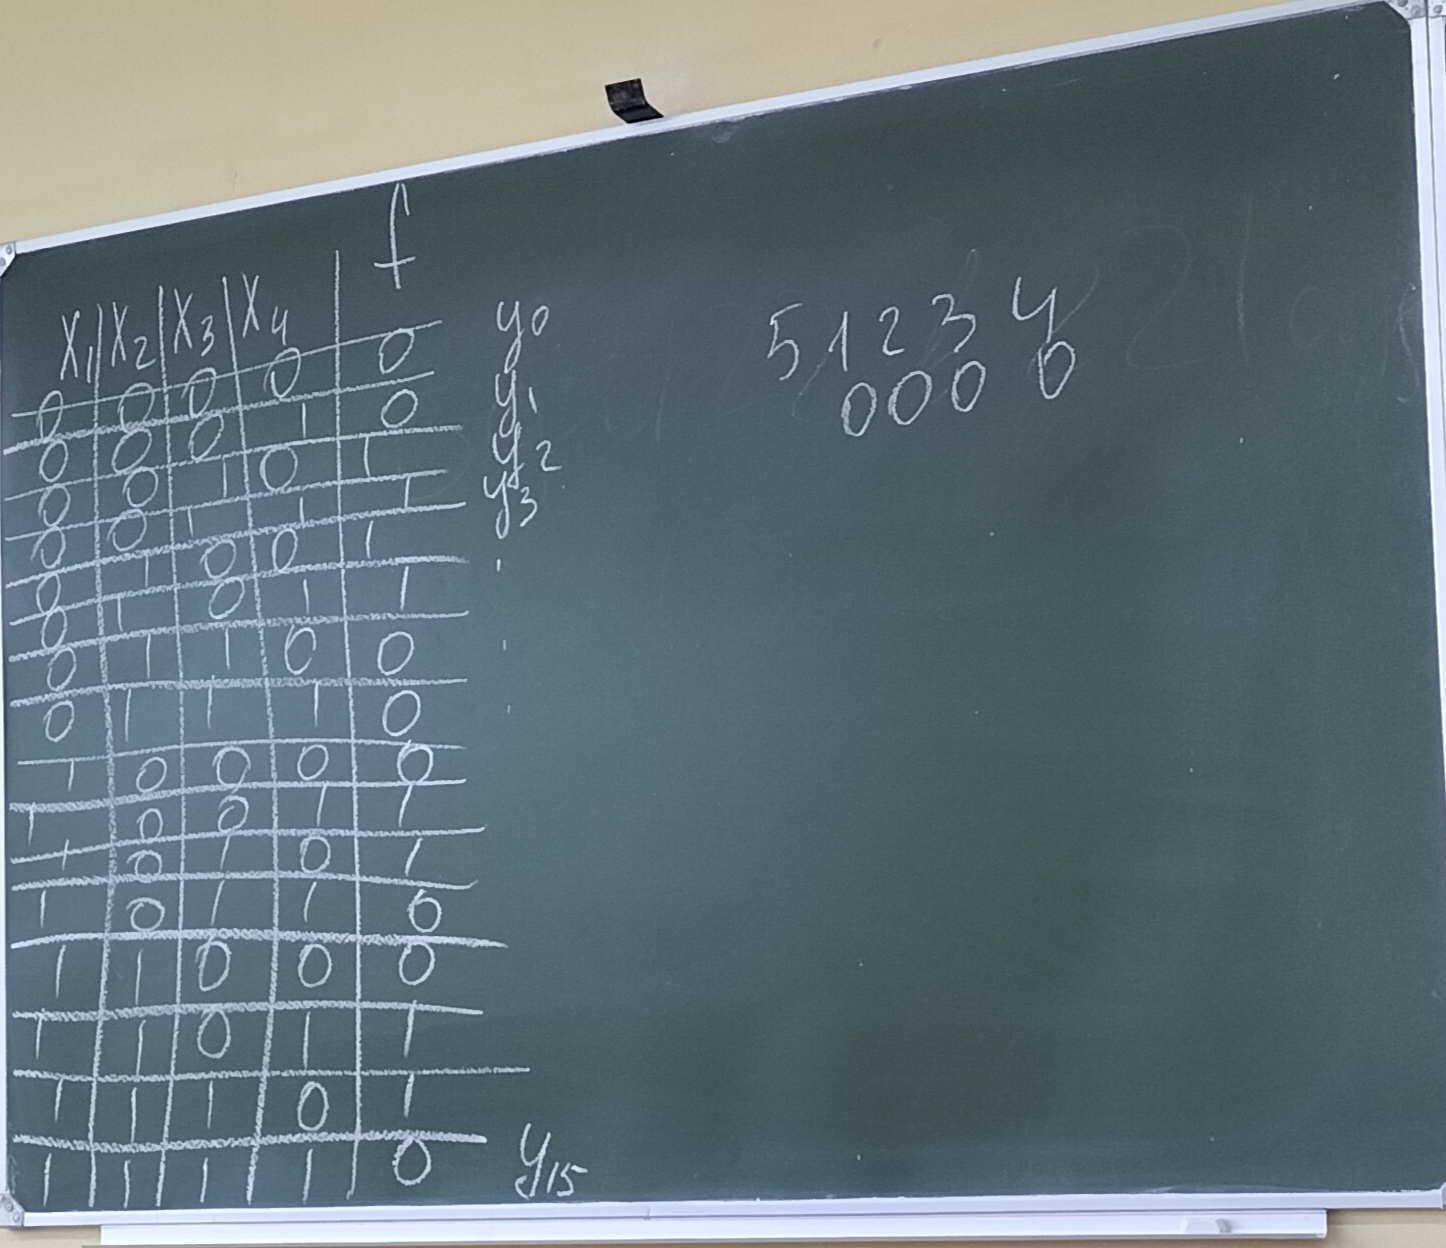
\includegraphics[width=\textwidth]{image_1.jpg}

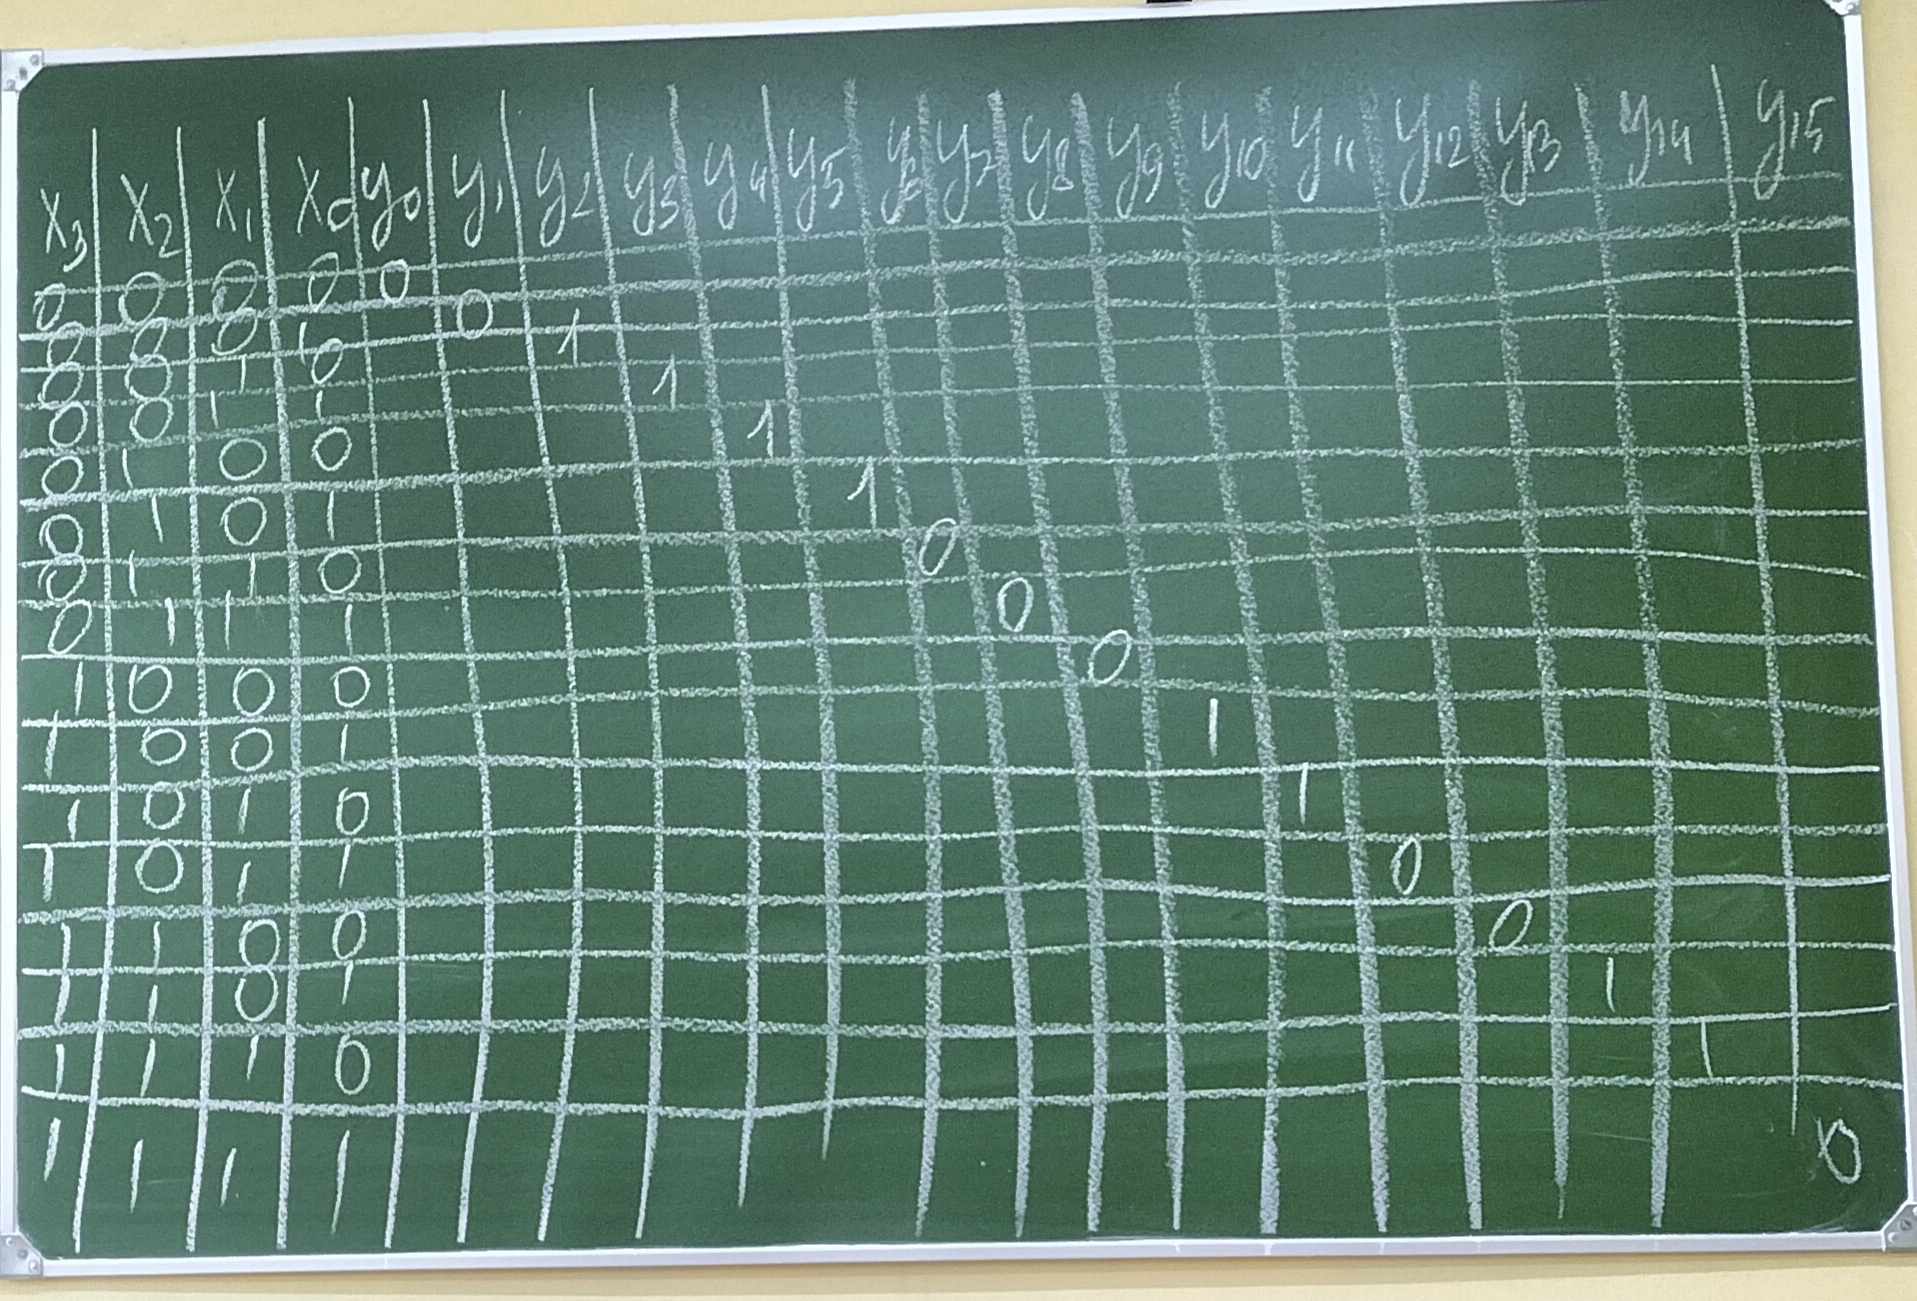
\includegraphics[width=\textwidth]{image_2.jpg}

Показать работоспособность - попереключать ключики - показать, что лампчка зажигается.

\end{flushleft}

\pagebreak
\section{Вычислительная техника - 31.10.2022}

\subsection{Последовательные цифровые устройства}

\begin{flushleft}

\textbf{Цифровые устройства} называются \textbf{последовательными}, если его входные сигналы зависят не только от текущих значений входных сигналов, но и от последовательности значений входных сигналов, поступивших на входы в предшествующие моменты времени, которые фиксируются с помощью элементов памяти.

\hfill

Эти устройства называются также цифровыми автоматами, конечными автоматами или автоматами с памятью.

\hfill

Примеры: триггеры, регистры, счетчики.

\pagebreak
\subsubsection{Триггеры}

\textbf{Триггером} называют устройство, которое может находиться неограниченно долго в одном из двух состояний устойчивого равновесия и переходить из одного состояния в другое под воздействием входного сигнала. Состояние триггера определяют по выходному сигналу В нем может храниться либо 0, либо 1.

\hfill

Входы триггера подразделяются на \textbf{информационные} и \textbf{управляющие} (вспомогательные). Сигналы, поступающие на информационные входы, \textbf{управляют состоянием} триггера. Сигналы на управляющих входах используются для \textbf{предварительной установки} триггера в требуемое состояние.

\hfill

Информационные входы триггера принято обозначать буквами \textbf{S, R, J, K, D, T}, а управляющие входы \textbf{C и V}

\paragraph{Классификация}

По \textbf{функциональным возможностям} триггеры разделяются на:

\begin{enumerate}
    \item триггер с раздельной установкой состояния 0 и 1 (RS-триггер)
    \item триггер с приемом информации по одному входу D (D-триггер или триггер задержки)
    \item триггер со счетным входом (T-триггер)
    \item универсальный триггер с информационными входами J и K (JK-триггер)
\end{enumerate}

По \textbf{способу приема информации}:

\begin{enumerate}
    \item \textbf{асинхронные триггеры} воспринимают информационные сигналы и реагируют на них в момент появления на входах триггера
    \item \textbf{синхронные триггеры} реагируют на информационные сигналы при наличии разрешающего сигнала на специальном управляющем входе C, называемом входом синхронизации
    \begin{enumerate}
        \item триггеры со \textbf{статическим управлением} по входу С воспринимают информационные сигналы при подаче на C-вход уровня 1 или 0
        \item триггеры с \textbf{динамическим управлением} по входу C воспринимают сигналы при изменении сигнала на C-входе
    \end{enumerate}
\end{enumerate}

\paragraph{Ключевые характеристики}

Триггеры \textbf{характеризуются} быстродействием, чувствительностью, потребляемой мощностью, помехоустойчивостью, функциональными возможностями.

\textbf{Быстродействие} определяется максимальной частотой переключения состояний триггера.

\textbf{Чувствительность} триггера определяется наименьшим напряжением на входе, при котором происходит переключение.

\textbf{Помехоустойчивость} характеризует способность триггера нормально работать в условиях помех.

\textbf{Функциональные возможности} триггера характеризуются числом входных сигналов.

\paragraph{Виды триггеров}

\subparagraph{Асинхронный RS-триггер} \textbf{с прямыми входами}

имеет два информационных входа $R$ и $S$, используемые для установки собствено $0$ и $1$, а также два выхода - прямой $Q$ и инверсный $Q$.

Быстродействие асинхронного RS-триггера определяется задержкой установки его состояния $T$, равной сумме задержек передачи сигнала через цепочку логических элементов $t$ в каждом. В данном случае $T = 2t$

\begin{SCfigure}[0.5][h]
\caption{Логическая схема асинхронного RS-триггера с прямыми входами}
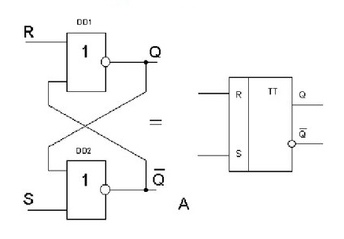
\includegraphics[width=0.6\textwidth]{assets/rs_direct.jpg}
\end{SCfigure}

\pagebreak
\subparagraph{Асинхронный RS-триггер} \textbf{с инверсными входами}

Формула: $Q^{t + 1} = S^{t} + Q^{t} * \overline{R^{t}}$

Таблица состояний триггера в моменты $t + 1$ может быть задана с помощью карты Карно.

\begin{SCfigure}[0.5][h]
\caption{Логическая схема асинхронного RS-триггера с инверсными входами}
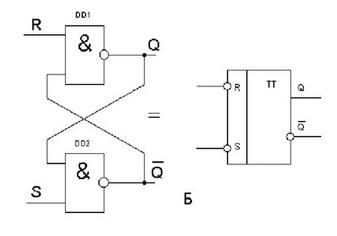
\includegraphics[width=0.6\textwidth]{assets/rs_invert.jpg}
\end{SCfigure}

\subparagraph{Синхронный RS-триггер}

Формула: $Q^{t + 1} = \overline{R^{t}} Q^{t} + \overline{C^{t}} Q^{t} + C^{t} S^{t}$

При $C = 0$ выходы логических элементов схемы $1$ принимают значение $1$ и не зависят от входных сигналов $S$ и $R$. При $C = 1$ входные логические схемы $1$ открыты для передачи информационных сигналов $R$ и $S$ на выходы асинхронного $RS$-триггера

\begin{SCfigure}[0.5][h]
\caption{Логическая схема cинхронного RS-триггера}
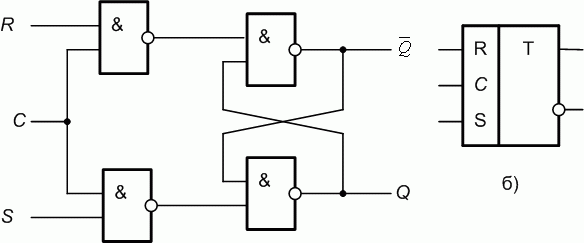
\includegraphics[width=0.6\textwidth]{assets/synchronous_rs.png}
\end{SCfigure}

\pagebreak
\subparagraph{D-триггер}

Триггер D-типа или триггер-задержка это синхронный триггер с одним информационным входом D, реализующий логическую функцию $Q^{t + 1} = C^{t} D^{t} \overline{C^{t}} Q^{t}$, то есть значение сигнала на входе $Q$ триггера на $t + 1$ такте (при $Ct = 1$) определяется значением входного сигнала $D$ на предыдщуем такте. Основное назначение $D$-триггер заключается в задержке информации на один такт.

\begin{SCfigure}[0.5][h]
\caption{Логическая схема D-триггера}
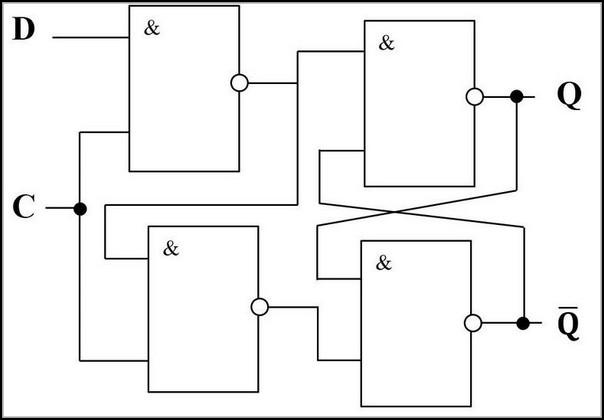
\includegraphics[width=0.6\textwidth]{assets/d_trigger.jpg}
\end{SCfigure}

\subparagraph{Двухступенчатый D-триггер}

В двухступенчатом триггере устраняется противоречие между процессами хранения старой и приема новой информации. Это дает возможность построения синхронных автоматов без опасных временных состояний. Позволяет обеспечить высокую надежность функционирования триггеров с внутренними цепями обратной связи.

Двухступенчатые D-триггеры обладают расширенными функциональными возможностями, например при соединении инверсного входа $Q$ со входом $D$ образуется триггер $T$-типа или триггер со счетным входом

\begin{SCfigure}[0.5][h]
\caption{Логическая схема двухступенчатого D-триггера}
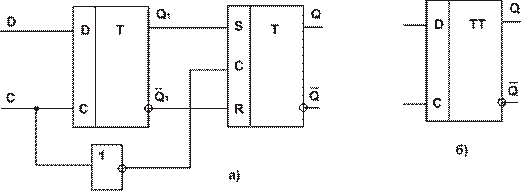
\includegraphics[width=0.6\textwidth]{assets/two_stage_d_trigger.png}
\end{SCfigure}

\pagebreak
\subparagraph{Универсальный JK-триггер}

JK-триггер отличается от синхронного RS-триггера тем, что не имеет запрещенных комбинаций сигналов на входах $J$ и $K$. Кроме того, при $J = K = 1$ триггер изменяет свое состояние на противоположное, т.е. работает как триггер со счетным входом.

Схема JK-триггера состоит из двух асинхронных RS-триггеров с инверсными входами и двух комбинационных устройств, каждое из которых содержит две схемы И-НЕ с тремя входами каждая.

На основе JK-триггера можно построить триггер D-типа. Для этого информационный сигнал $D$ подается на J-вход, а на вход K сигнал $D$ подается через инвертор.

\begin{SCfigure}[0.5][h]
\caption{Логическая схема универсального JK-триггера}
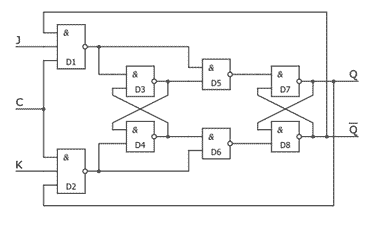
\includegraphics[width=0.6\textwidth]{assets/jk_trigger.png}
\end{SCfigure}

\subparagraph{T-триггер}

Может быть получен из JK-триггера при соединении обоих информационных входов $J$ и $K$, и при подаче на них уровня $1$. В качестве счетного входа $T$ используется вход $C$. При подаче сигнала на вход $C$, T-триггер будет переключаться в состояние, противоположное предыдущему.

Разновидностью T-триггера является TV-триггер, в котором вход $V$ является управлющим. При $V = 1$ TV-триггер превращается в T-триггер. При $V = 0$ TV-триггер сохраняет свое состояние неизменным.

\begin{SCfigure}[0.5][h]
\caption{Логическая схема T-триггера на основе JK-триггера}
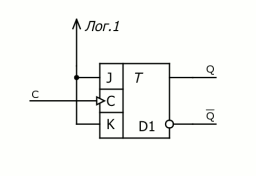
\includegraphics[width=0.6\textwidth]{assets/t_trigger.png}
\end{SCfigure}

\subparagraph{Синхронный триггер с динамическим управлением}

Синхронный триггер с динамическим управлением по входу C воспринимает информацию для изменения состояния лишь тогда, когда на C-входе совершается переход с уровня $0$ на уровень $1$, либо наоборот.

Если при $C = 0$ на информационные входы схемы на элементах И-НЕ поступили какие-либо уровни $S$ и $R$, то при смене уровня на входе C с $0$ на $1$ на выходе элемента Э1 образуется $0$, который поступает на вход элемента Э3 и обеспечивает на его выходе уровень $1$ независимо от последующих значений уровня на входе $S$.

Вход $S$ логически отключается и никакие изменения уровней на входах $S$ и $R$ триггер не воспринимает, пока не произойдет на входе C переход с уровня $0$ на урвоень $1$. Аналогично можно построить схему RS-триггера с динамическим входом на элементах ИЛИ-НЕ. Здесь информация воспринимается триггером со входов S и R при смене уровней $C = 1$ на $C = 0$

\begin{SCfigure}[0.5][h]
\caption{Логическая схема синхронного RS-триггера с динамическим управлением}
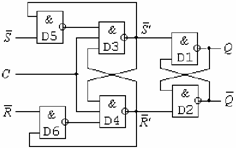
\includegraphics[width=0.6\textwidth]{assets/synchronous_rs_trigger.png}
\end{SCfigure}

\subparagraph{D-триггер с динамическим управлением}

Прием в триггер информации со входа $D$ происходит в момент смены на входе $C$ уровня $0$ на уровень $1$.

\begin{SCfigure}[0.5][h]
\caption{Логическая схема синхронного D-триггера с динамическим управлением}
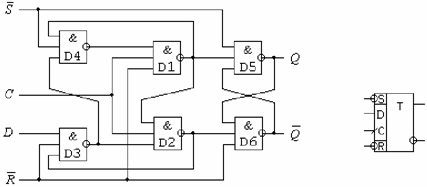
\includegraphics[width=0.6\textwidth]{assets/synchronous_d_trigger.png}
\end{SCfigure}

\subsubsection{Регистры памяти}

Регистром называется устройство, предназначенное для выполнения операций приема, хранения и передачи слов в двоичном коде. По способу хранения информацию различаются статические и динамические регистры. По типу записи информации регистры подразделяются на параллельные, последовательные и последовательно-параллельные. На основе таких регистров осуществляются операции преобразования последовательного кода в параллельный и наоборот.

\hfill

Регистр с параллельным приемом и выдачей информации называется регистром памяти. Он позволяет записывать, хранить и в нужный момент выдавать информацию в прямом или обратном коде. Регистры памяти могут быть построены на RS-, D- или JK-триггерах.

\hfill

При подаче управляющего импульса на шину «Сброс» все триггеры устанавливаются в нулевое состояние. Ввод новой информации в регистр осуществляется через ячейки И, связанные с входными шинами.

Для записи информации, подведенной к входным шинам, подается управляющий импульс на шину «Ввод». При этом срабатывают те ячейки И, на входных шинах которых действует сигнал $1$. Под действием импульсов, появляющихся на выходах ячеек И, соответствующие триггеры будут установлены в состояние $1$.

Вывод информации из регистра осуществляется через элементы И, связанные с выходами триггеров. Для выдачи информации в инвертированном коде, когда все единицы заменяются нулями, а нули единицами, необходимо подать управляющий импульс на шину «Обращение кода», соединенную со счетными входами триггеров.

\end{flushleft}


\end{document}
